\chapter{Experimenteller Aufbau}
\label{chap:Aufbau}
Im Folgenden wird zunächst die Methodik und anschließend der Aufbau des Experiments und das Zusammenwirken der verschiedenen Komponenten erläutert. Die meisten Elemente wurden nicht im Rahmen dieser Arbeit verbaut, sondern sind bereits von vorherigen Arbeiten der Arbeitsgruppe vorhanden. Diese sind in \cite{Holzte} beschrieben. Abbildung \ref{fig:Aufbau} zeigt den schematischen Aufbau der Vakuumkammer und des Experiments.

\section{Methodik}
Im Folgenden wird das Grundprinzip der Anlage erläutert und erklärt, wie diese für die Charakterisierung von Treibstoffen in einem RIT verwendet werden kann.

\subsection{Ionisation} 
Die Ionisation des Treibstoffs und dessen Beschleunigung können in einem RIT in der Regel als voneinander getrennte Prozesse betrachtet werden \cite{ion}. Um das Verhalten eines Gases, und somit auch seine Effizienz als Treibgas in einem RIT zu bewerten, ist es wichtig das im Entladungsgefäß gezündete Plasma möglichst gut zu verstehen. Die Ionisation wird nicht in einem RIT über Magnetfelder eingeleitet, sondern mit einer Elektronenkanone. Da primär die Wirkungsquerschnitte und die Zusammensetzung der Menge von erzeugten Ionen von Relevanz sind, kann die Testanlage so deutlich simpler gestaltet werden und es wird kein Radiofrequenzgenerator benötigt. Basierend auf früheren Arbeiten der Arbeitsgruppe für Ionentriebwerke an der JLU, wird in dieser Arbeit die bestehen Anlage \textit{ZeroB} ausgebaut. Für das Messen der relevanten Größen müssen die Ionen nachgewiesen und identifiziert werden können. Dafür soll zunächst ein neuer Detektor installiert werden, der eine höhere Auflösung und einen größeren Durchmesser aufweist. Mithilfe des Detektors kann der Zeitpunkt des Auftreffens und der Ort einzelner Ionen bestimmt werden. Damit die Ionen konsistent auf den Detektor treffen, werden sie mit einem elektrischen Feld beschleunigt und ihre Flugzeit gemessen. Der Aufbau der Anlage ähnelt dem von Straub et al. aus \cite{Straub}, der bereits in den 90er-Jahren viele Flugzeitspektren und Wirkungsquerschnitte mittels Elektronenstoßionisationen aufgenommen hat. Eine genaue Beschreibung des Experimentellen Aufbaus ist in Kapitel \ref{chap:Aufbau} zu finden.

Um alle Mehrteilchen- und Mehrfachstoßeffekte in der Praxis vernachlässigen zu können, werden die Paramter, also der Gasdruck, die Pulslänge und Frequenz, sowie der Extraktionsstrom der Elektronenkanone so gewählt, dass pro Puls im Mittel nur ein Stoß stattfindet. Das wird das durch eine kurze Strahlzeit erreicht und über die Rate der Signale am Detektor überprüft. Diese wird bei allen Messungen auf unter 300 Hz gehalten, da, wie im Folgenden noch genau beschrieben, ein Anteil von etwa 1/10 der Ionen detektiert werden können und die Kanone mit einer Rate von etwa 3 kHz gepulst wird.

\subsection{Flugzeitmessung}
Eine Flugzeitmessung ist eine der zentralen Methoden in der Massenspektroskopie. Sie basiert darauf die Flugzeit einzelner zuvor beschleunigter Teilchen für eine bestimmte Strecke im Vakuum zu messen. In dieser Arbeit wird über eine Flugzeitmessung das Masse-zu-Ladungsverhältnis einzelner Ionen bestimmt. Im Folgenden wird gezeigt, wie die Geschwindigkeit und Flugzeit von Ionen einen Rückschluss auf ihre Masse und Ladung geben.

Durch Anlegen eines elektrischen Feldes, können elektrisch geladene Teilchen über die Coulombkraft beschleunigt werden. Die Beschleunigung $a$ welche Ionen mit der Ladung $q_i$ und Masse $m_i$ erfahren, wenn sie sich in einem elektrischen Feld mit der Feldstärke $E$ befinden wird in Formel \ref{eq:beschleunigung} beschrieben: 
\begin{equation}
    \label{eq:beschleunigung}
    a = \frac{q_i}{m_i} \cdot E.
\end{equation}
Die Flugzeit $t_f$ der Ionen über einer festen Strecke $d$ im Feld kann dann wie folgt beschrieben werden:
\begin{equation}
    t_f = \sqrt{\frac{m_i}{q_i}} \cdot \sqrt{\frac{2d}{E}} = \sqrt{\frac{m_i}{q_i}} \cdot \sqrt{\frac{2}{U}} \cdot d.
\end{equation}
Hieraus ist offensichtlich, dass eine Variation der Flugzeit allein von ihrem Masse-zu-Ladungsverhältnis $\frac{m_i}{q_i}$ abhängt, wenn die Spannung $U$ und der Abstand $d$ konstant bleiben. Treten die Ionen aus dem Feld aus fliegen sie weiter mit konstanter Geschwindigkeit, unabhängig ihrer Eigenschaften. Ein Flugzeitspektrum zeigt dann höher geladene Ionen desselben Elements mit einer geringeren Flugzeit. In der Theorie ist dises Spektrum diskret für verschiedene Masse zu Ladungsverhältnisse, im Labor sind die Peaks jedoch etwas ausgedehnt, wie in Abbildung \ref{fig:rest_tof} zu sehen. Das liegt daran, dass der Ort der Entstehung der Teilchen nicht genau gemessen werden kann, sondern von der Breite des Elektronenstrahls abhängt.

Um die Flugzeit experimentell zu bestimmen, wird ein Start- und Stoppsignal benötigt. Der Startzeitpunkt muss den Eintritt in das elektrische Feld markieren und der Stoppzeitpunkt das Auftreffen auf einen Detektor. Kritisch ist dabei, die Flugzeit mit hinreichender Genauigkeit unabhängig vom Ion zu bestimmen. Typische Flugzeiten sind in diesem Aufbau in der Größenordnung von Mikrosekunden. Wie auch in der Arbeit von Straub et al. wird ein Pulsgenerator verwendet, der einen Hochspannungspuls auf einer Ablenkplatte, und damit das elektrische Feld zur Beschleunigung der Ionen erzeugt. Der Puls, der diese Spannung triggert wird auch als Startsignal verwendet. Diese Flugzeitmessung wird in Kapitel \ref{chap:Sim} auch ausgiebig simuliert.

\begin{figure}
    \centering
    \hspace*{-.8cm}
    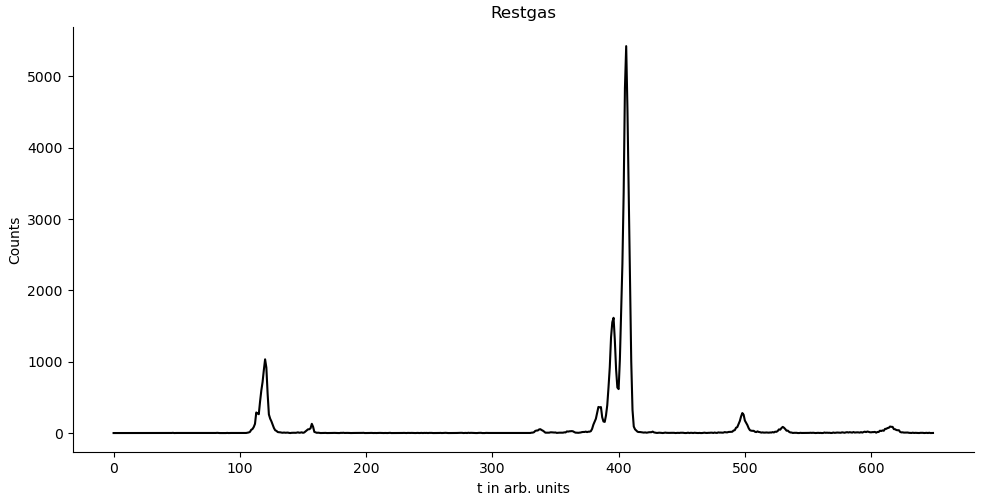
\includegraphics[width=.95\textwidth]{Restgas_tof.png}
    \caption[Flugzeitspektrum der Restgase]{Unskaliertes Flugzeitspektrum der Restgase in der Vakuumkammer. Die Zeitachse ist in willkürlichen Einheiten angegeben. Zur Bestimmung der Masse-zu-Ladungsverhältnisse muss das Spektrum anhand einiger Annahmen skaliert werden.}
    \label{fig:rest_tof}
\end{figure}

\section{Vakuumkammer und Druckmessung}
Die Experimente finden in einer Vakuumanlage mit einer kubischen Hauptkammer statt, von der alle anderen Komponenten abzweigen. Die Kammer hat eine Seitenlänge von 30 cm. Sie besteht auch $\mu$-Metall, damit das Magnetfeld im Inneren der Kammer minimal ist. Das ist wichtig, damit die Elektronen nicht von äußeren Magnetfeldern abgelenkt werden. Die Abschirmung reduziert das Magnetfeld auf unter 15 mG \cite{Holzte}. Die Kammer ist mit einer Turbomolekularpumpe und einer Vorpumpe ausgestattet. Diese können ein Vakuum in der Größenordnung von 10$^{-8}$ mBar nach Ausheizen der Kammer erreichen. Am überliegenden Flange ist ein kapazitiver Drucksensor angebracht, der \textit{MKS Barathron 690A.1TRB}. Dieser misst den Druck bis zu 3 $\cdot 10^{-6}$ mbar mit einer Genauigkeit von 0,08 \%. Dafür wird das Restgas auf \ang{45}C aufgeheizt. Die Temperaturdifferenz zum restlichen Aufbau muss später berücksichtig werden. Ein zweiter Druckmesser ist ein Bayard-Alpert-Glühkathoden-Ionisationsvakuummeter, welches Drücke bis unter $10^{-8}$ mbar messen kann. Dieses dient als Referenz, damit das genauere kapazitive Messystem genullt werden kann und erweist sich als ausgesprochen praktisch bei der Arbeit mit dem Hochvakuum.
Zum Einlassen der zu untersuchenden Gase ist ein temperaturgesteuertes Regelventil verbaut. Dieses kann sehr empfindlich eingestellt werden, sodass der Gasdruck im Betrieb genau bestimmt werden kann. An das Ventil ist dann eine Gasflasche über einen Druckminderer angeschlossen. Das Gas kann so direkt in die Hauptkammer eingelassen werden, wo dann die Ionisation stattfindet.

\begin{landscape}
    \begin{figure}
        \centering
        \vspace{-1.5cm}\hspace{-4cm}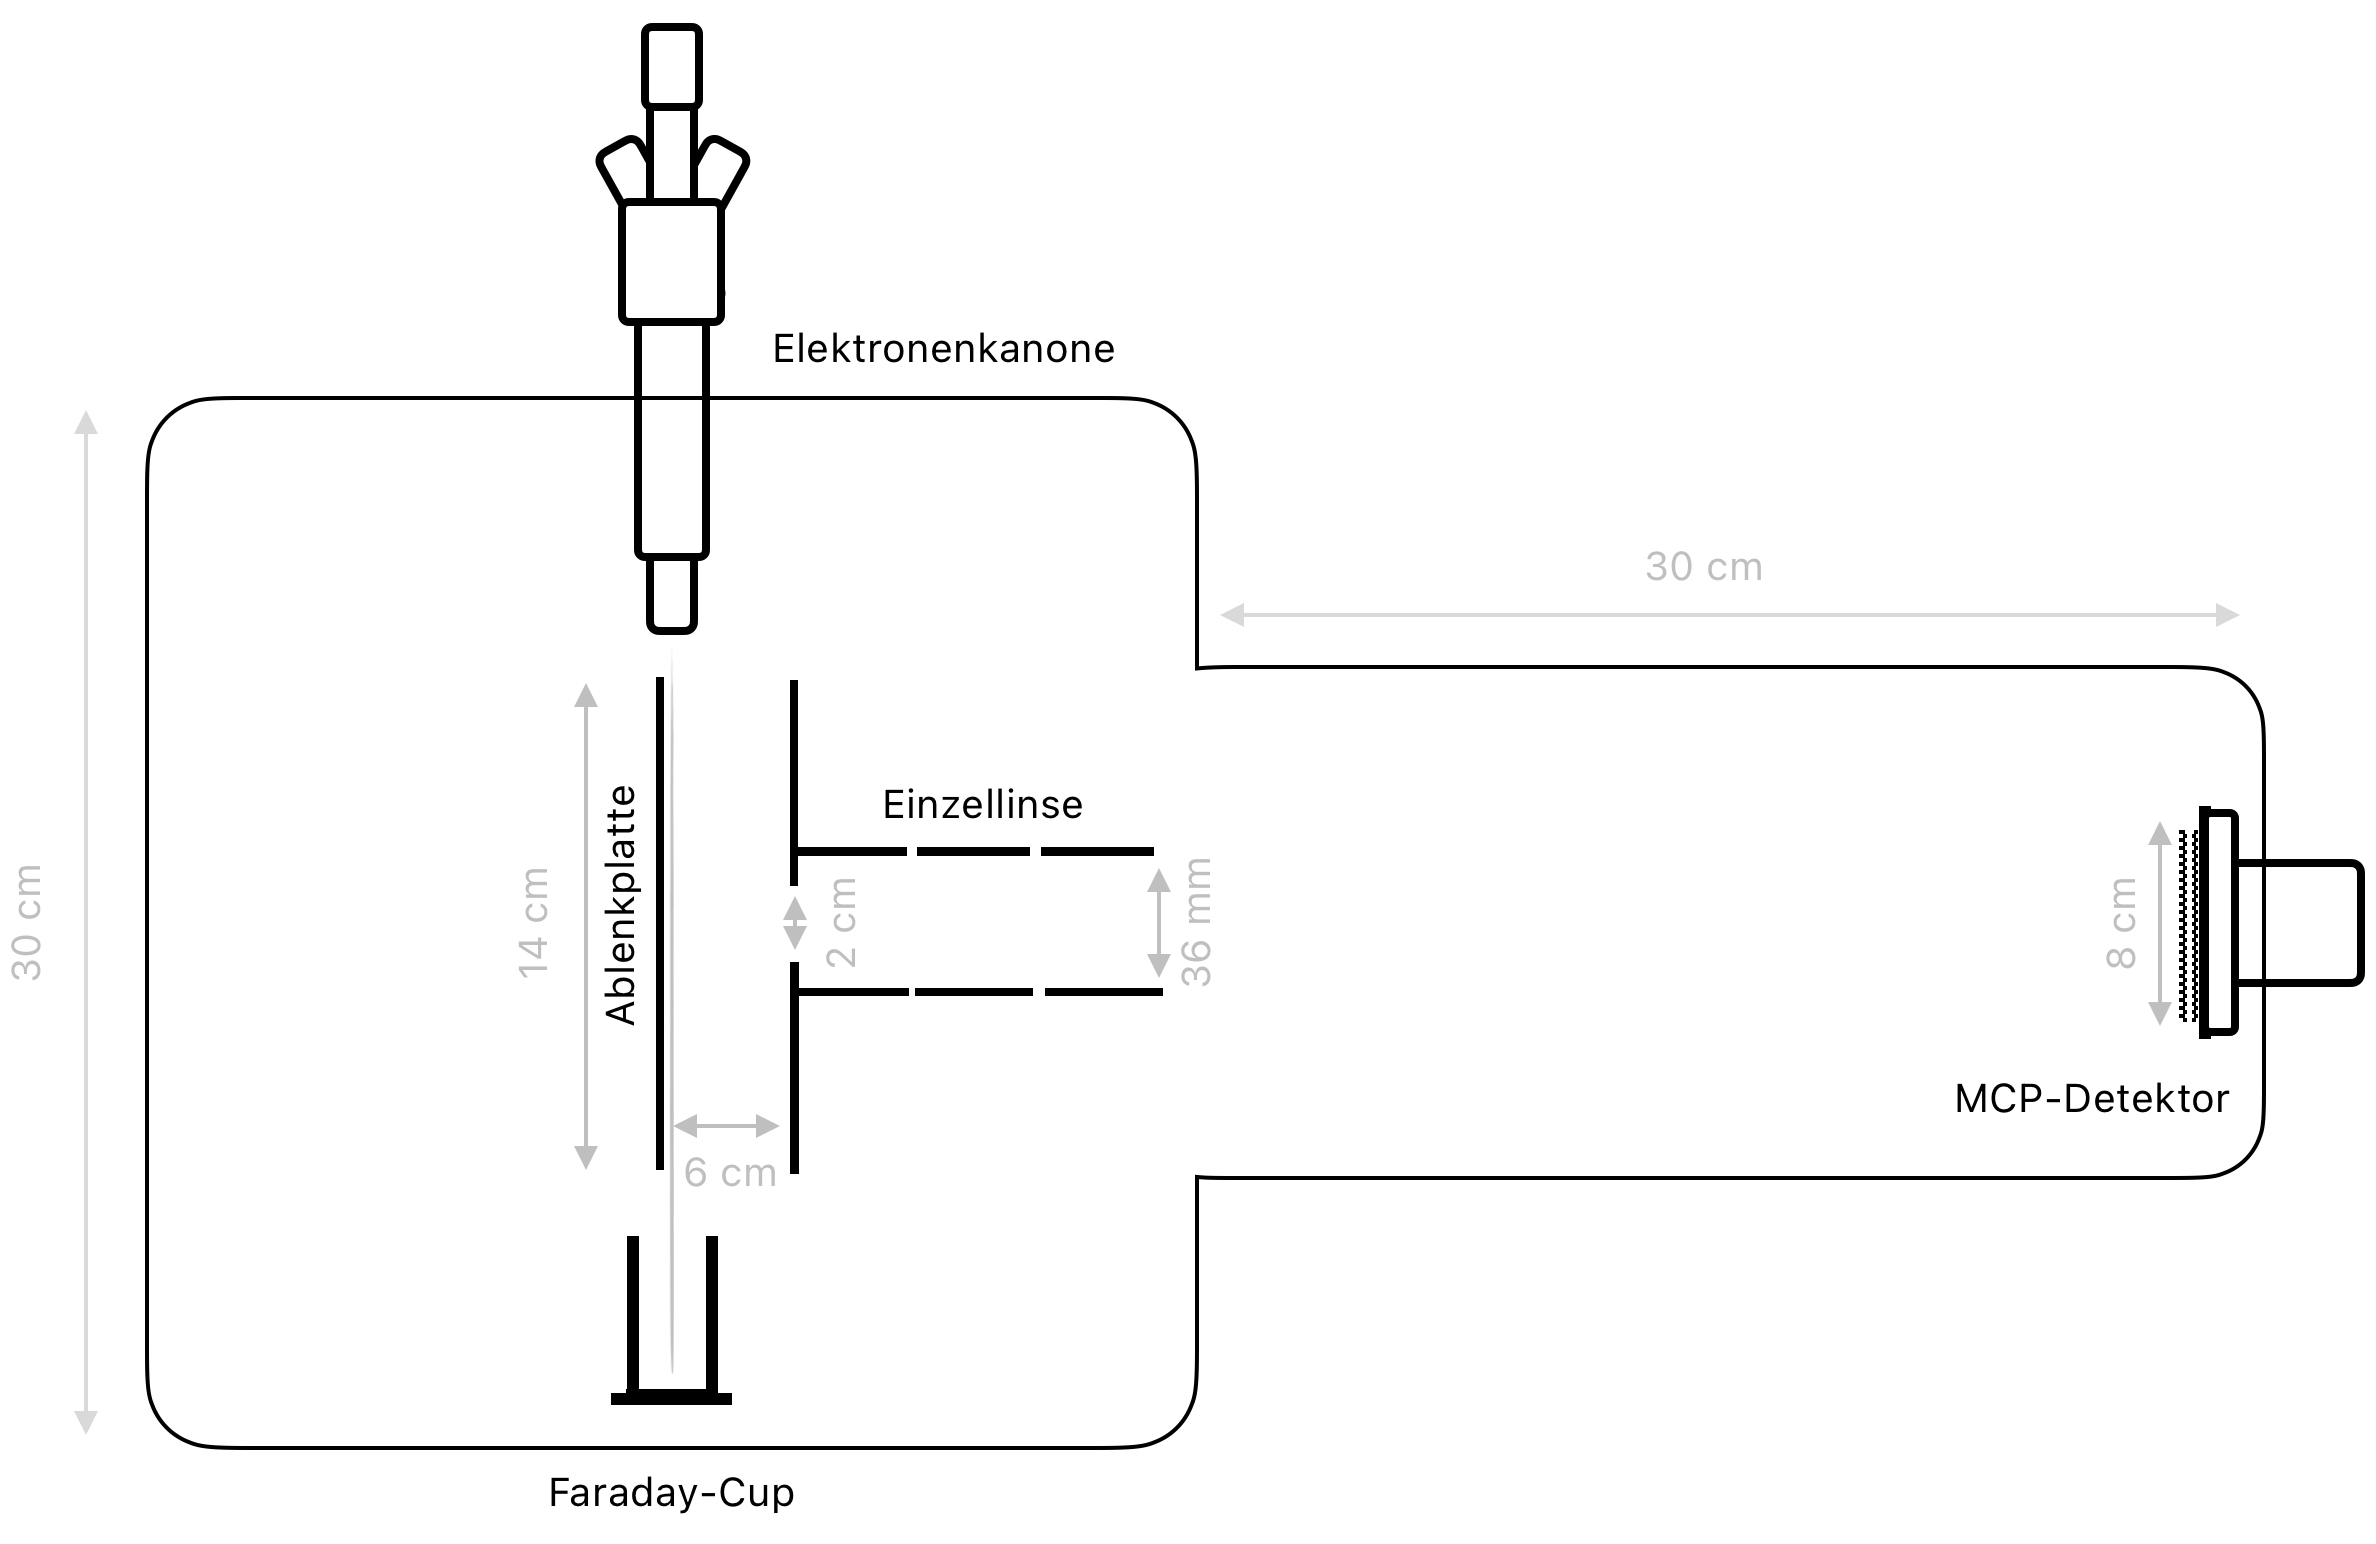
\includegraphics[width=1.4\textwidth]{SchematischerAufbau.png}
        \caption[Schematischer Aufbau des Experiments]{Schematischer Aufbau des Elektronenstoß-Experiments in der Vakuumkammer \textit{Zero-B}. Die Elektronen werden von der Elektronenkanone erzeugt. Sie stoßen mit den Neutralgasteilchen und ionisieren diese durch Stoßionisation. Die entstehenden Ionen werden über ein elektrisches Feld von einem Plattenkondensator in Richtung der Detektorplatten beschleunigt und passieren dabei eine Einzellinse.}
        \label{fig:Aufbau}
    \end{figure}
\end{landscape}

\section{Elektronenstrahl und Ablenkplatte}
Für die Elektronenstoßionisation ist eine Heizkathoden-Elektronenkanone an einer der seitlichen Flange verbaut. Dabei handelt es sich um ein energieverstellbares Gerät von Kimball Physics, die \textit{ELG-2/EGPS-1022}. Es kann einen Energiebereich zwischen 1 eV bis 2 keV abdecken. Der Strahl ist in der Ebene ablenkbar und kann variabel fokussiert werden. Die thermische Energieschärfe der verschossenen Elektronen beträgt 0,5 eV bei der Verwendung einer Tantal-Heitzkathode. Außerdem ist es möglich die Kanone in einem gepulsten Betrieb zu benutzen, was für dieses Experiment benötig wird. Dabei werden die Elektronen von einer Gitterspannung abgebremst und nur über Spannungspulse für kurze Strahldauern durchgelassen. Die Frequenz darf 5 kHz nicht überschreiten. Einen Querschnitt der Elektronenkanone zeigt Abbildung \ref{fig:EGun}. Eingestellt werden kann die Kanone über eine mitgelieferte Steuerungseinheit. Um eine optimale Fokussierung zu finden, muss für jede Energie die Anoden- und Fokusspannung angepasst werden. Während dieser Arbeit stellte sich heraus, dass Elektronenkanone eine Reperatur braucht, da die Heizkathode nicht mehr ordnungsgemäß funktioniert.

\begin{figure}
    \centering
    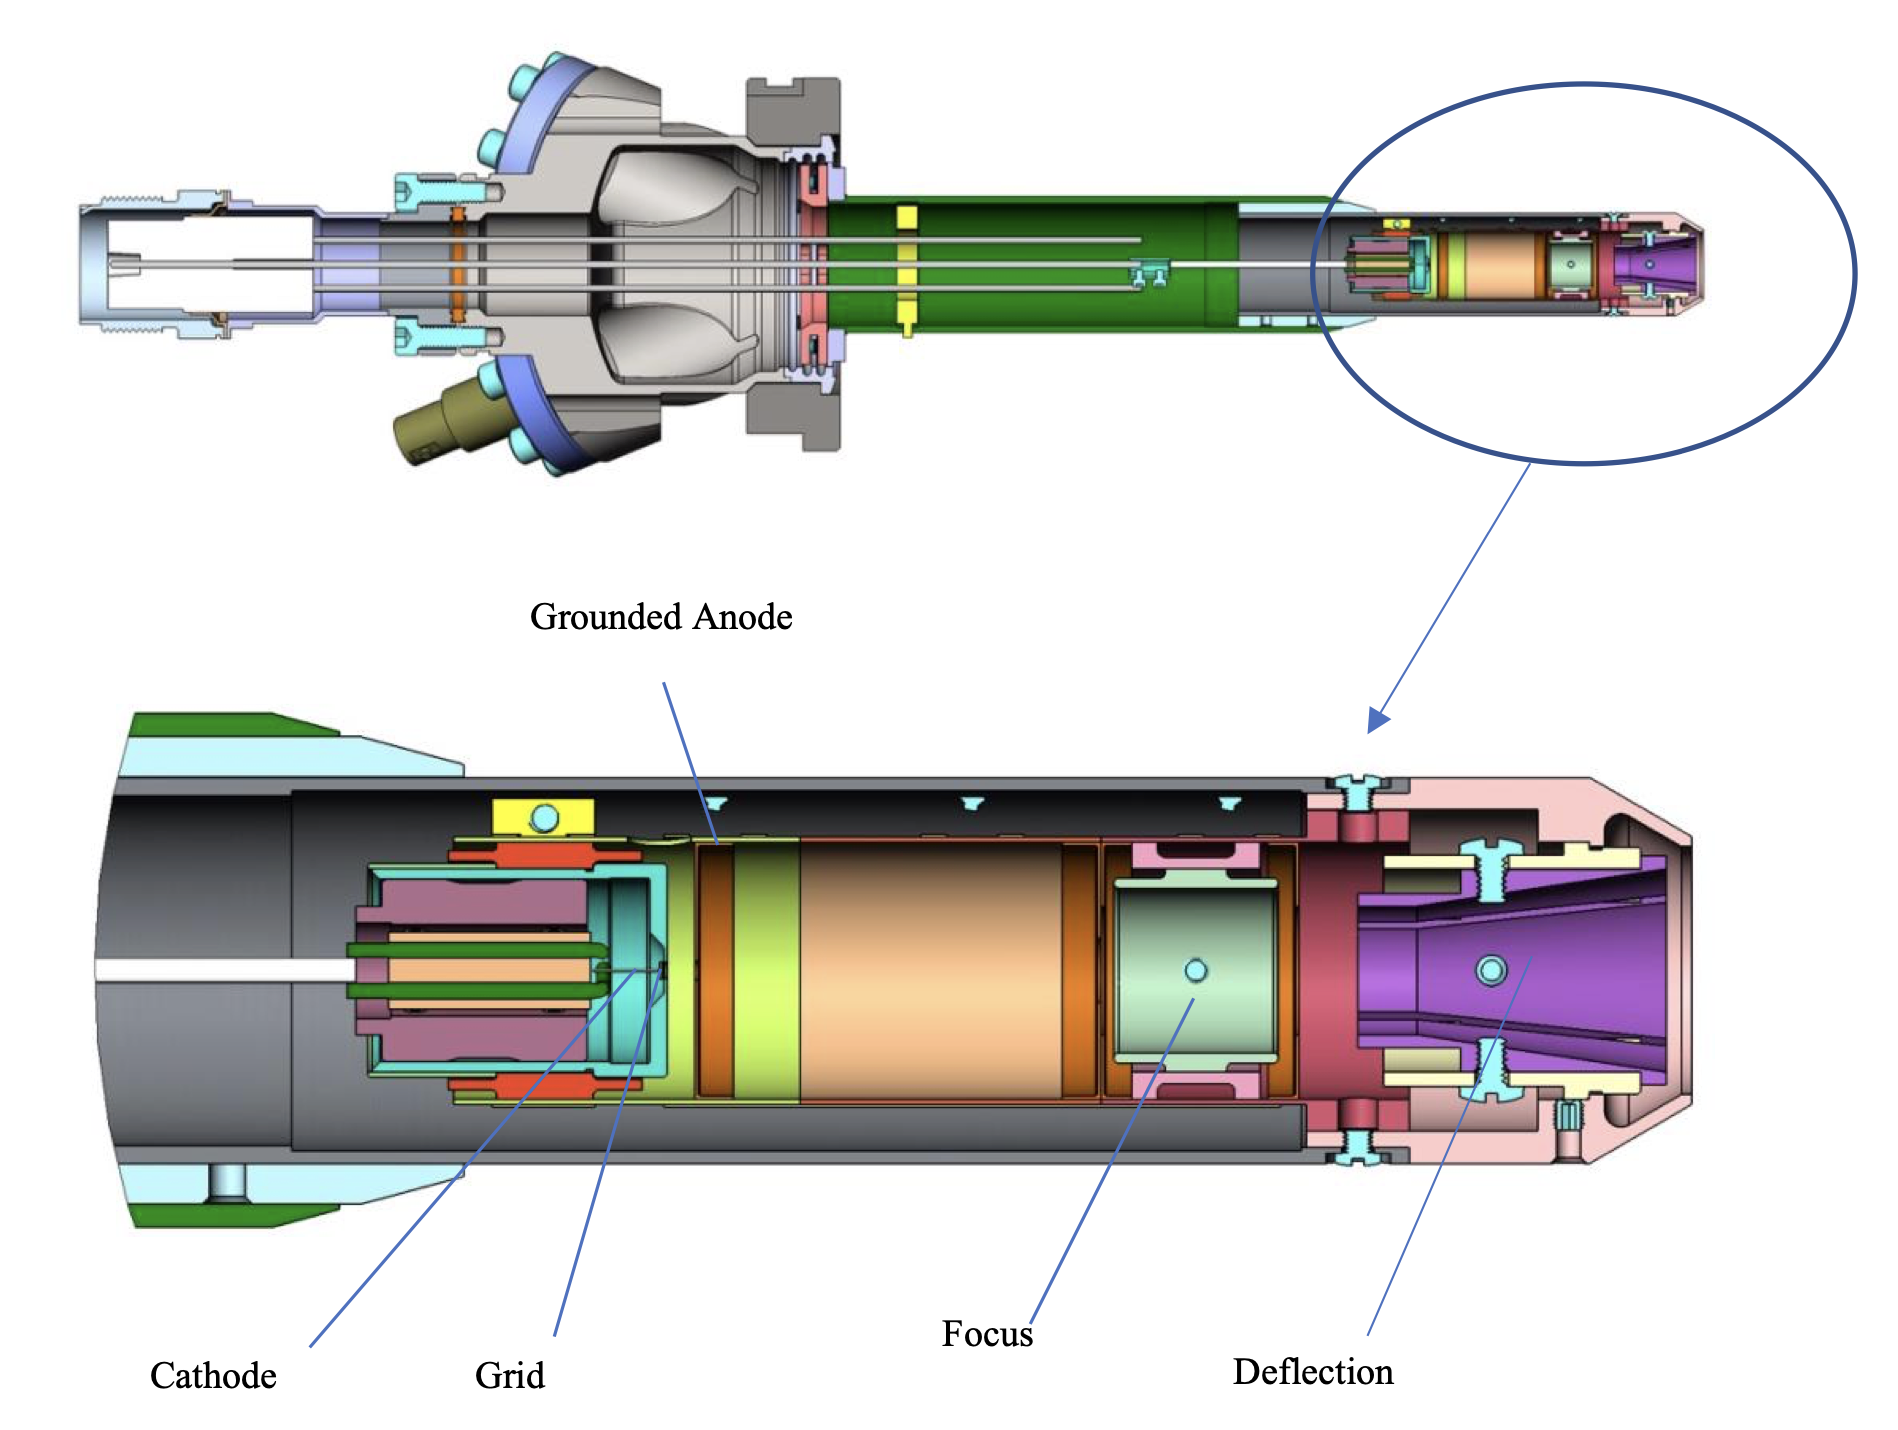
\includegraphics[width=.8\textwidth]{EGun.png}
    \caption[Querschnitt der Elektronenkanone]{Querschnitt der Elektronenkanone von Kimball Physics. Die Elektronen werden durch eine Heizkathode (Cathode) erzeugt und durch eine Gitterspannung (Grid) beschleunigt. Sie können fokussiert und abgelenkt werden.}
    \label{fig:EGun}
\end{figure}

Der Kanone gegenüber ist ein Faraday-Cup angebracht. Mit diesem kann die tatsächliche, momentane Elektronenstromstärke gemessen werden. Eine genaue Messung des Elektronenstroms ist für eine Messung des Wirkungsquerschnittes und für das Finden eines guten Arbeitspunktes für die Elektronenkanone essenziell. Der Faraday-Cup ist ein Metallzylinder, der von einem Isolator umgeben ist und dient als einfaches Ladungsgefäß. Er ist mit einem Elektrometer, dem \textit{DDPCA-300} von FEMTO, verbunden, welches den Strom und die Ladung auf dem Cup im Femto-Ampere und Pico-Coulomb Bereich messen kann. Für die Messung der Ladung ist es wichtig, dass die von der Elektronenkanone im gepulsten Betrieb akkumulierte Ladung dem Rauschen deutlich überwiegt. Deshalb ist es, besonders für geringe Elektronenenergien, lohnenswert den Elektronenstrom bestmöglich einzustellen und ein rauscharmes Kabel zu verwenden. Für diese Messung wurde ein besonders großer Faraday-Cup mit einem Durchmesser von 30 mm und einer Tiefe von ca. 80 mm verwendet. Das hat zwei Gründe: Zum einen ist die Fläche des Cups groß genug, um den gesamten Elektronenstrom aufzufangen - auch wenn er nicht perfekt fokussiert ist oder vom magnetischen Restfeld abgelenkt wurde, was essenziell für die Messung ist. Zum anderen ist die Tiefe des Cups möglichst groß gewählt, damit es unwahrscheinlicher ist, dass aus dem Cup durch Stoßionisation entstandene Ionen in die Kammer gelangen. Von dem sonst aus diesem Grund verwendeten Repeller-Ring wurde abgesehen, da das elektrische Feld Einfluss auf die Messung nehmen könnte.

In der Mitte der Kammer durchquert der Strahl einen zylindrischen Plattenkondesator, wobei er die Bodenplatte mit einem Abstand von etwa 1,5 cm parallel passiert. Auf der Bodenplatte kann über einen Hochspannungspulsgenerator (PVX-4130) ein elektrisches Feld angelegt, um die Ionisationsprodukte auf die Detektorplatten zu beschleunigen. Dieser kann hochfrequente Pulse von bis zu 6 kV mit einer Flankenanstiegszeit von wenigen Nanosekunden erzeugen. Der Spannungspuls wird leicht verzögert ausgelöst. Die Deckenplatte hat in der Mitte ein kreisförmiges Loch mit 2 cm Durchmesser, durch das die Ionen Richtung Detektor gelangen. Auf diesem befindet sich ein Goldnetz (88\% Transparenz), das Restfelder hinter dem Plattenkondensator reduzieren soll. Die Frotplatte des Detektors liegt, wie im nächsten Abschnitt genauer beschrieben, auf einem negativen Potenzial von -2,5 kV, so dass sich bei einem Spannungspuls von 4 kV und einem einfach geladenen Ion in etwa eine kinetische Energie $E_{kin} = e \cdot (U_{Detektor} - U_{Kondensator}) = 6,5$ keV ergibt. Ein 3D-Modell der Kammer mit dem Plattenkondensator ist in Abbildung \ref{fig:3D} zu sehen.

\begin{figure}
    \centering
    \hspace{-2.4cm}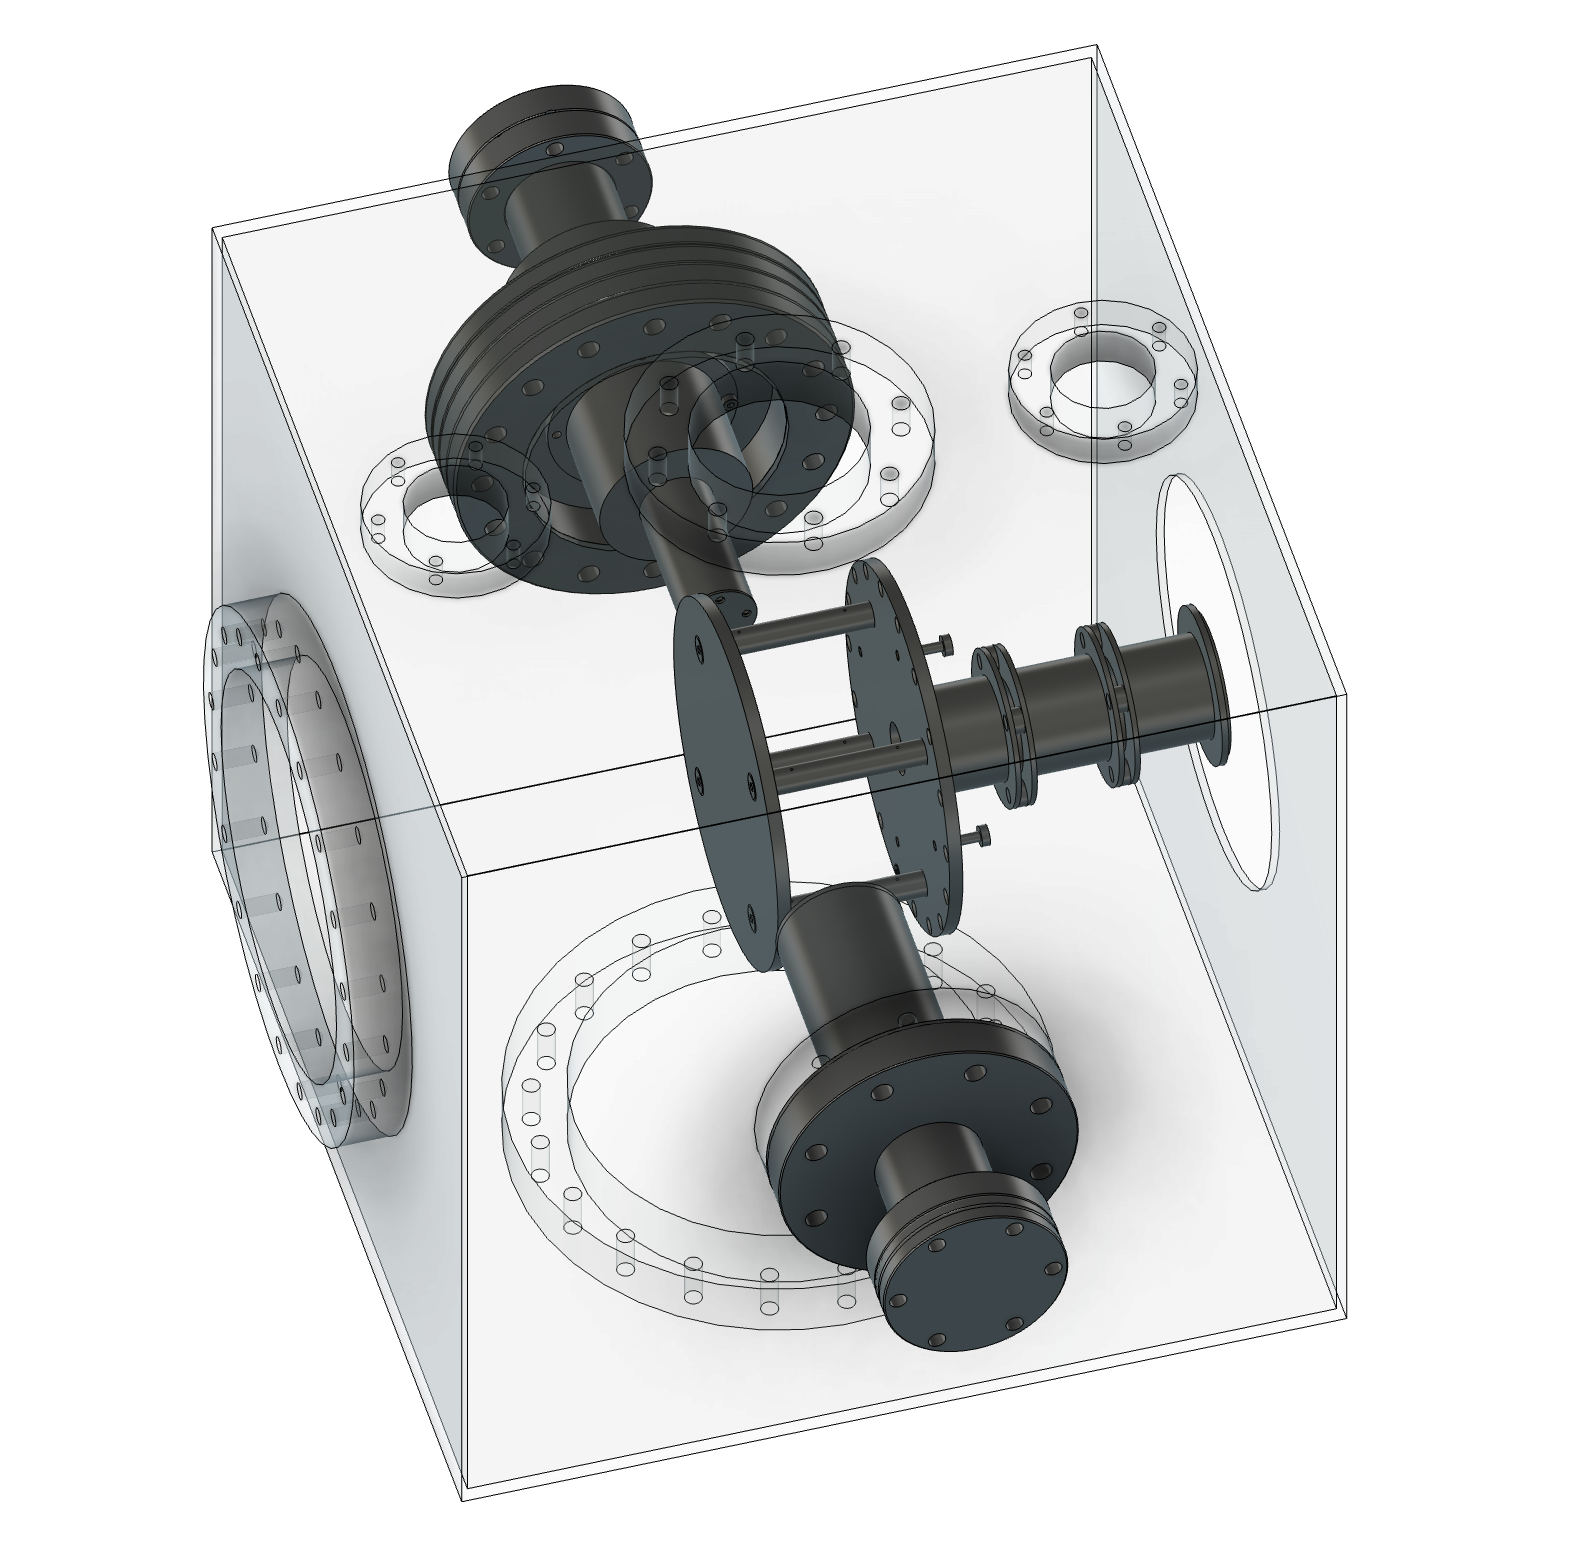
\includegraphics[width=1.2\textwidth]{Kammer_3D.png}
    \caption[3D-Modell der Vakuumkammer mit Plattenkondensator]{3D-Modell der Vakuumkammer mit Plattenkondensator. Auf der, der Kamera zugewandten Seite ist der Faraday-Cup zu sehen, gegenüber die Elektronenkanone. Der Strahl durchquert den zylindrischen Plattenkondensator in der Mitte und die Produkte werden durch eine elektrische Einzellinse (drei Zylinder, rechts) hindurch auf die Detektorplatten (nicht abgebildet) extrahiert. Durchsichtig abgebildet sind die Seitenwände der Kammer.}
    \label{fig:3D}
\end{figure}

\section{Detektorsystem}
Bei dem in dieser Arbeit verwendeten Detektor handelt es sich um einen positionssensitiven Mikrokanalplattendetektor (engl. \textit{micro channel plate detector}, MCP-Detektor) der Firma Roentdek. MCP-Detektoren sind eine verbreitete Detektortechnologie, die es ermöglicht den Auftreffzeitpunkt von einzelnen Ionen, Elektronen oder Photonen zu bestimmen. Mit einer Widerstandsanode kann die Position der durch die Platten verstärkten Signale anschließend bestimmt werden. So kann ein \textit{Bild} der detektierten Teilchen erzeugt werden. Im Versuchsaufbau schirmt das soeben erwähnte Goldnetz den Detektor von elektromagnetischen Störungen und Restfeldern ab. Die für den Detektor typischen Leistungsparameter sind in Tabelle \ref{tab:MCP} aufgeführt. Der für das Experiment verwendete Detektor ist ein \textit{delay-line} Detektor, genauer der \textit{DLD80} von Roentdek.

% table of typical values for MCP detectors
\begin{table}[h]
    \centering
    \caption{Von Roentdek angegebene typische Parameter für den MCP-Detektor}
    \begin{tabular}{c|c}
        Parameter & Wert \\
        \hline
        Aktive Fläche & 80 mm \\
        Effizienz & $>$ 50\% \\
        räumliche Auflösung & $<$ 0,1 mm \\
        Zeitauflösung & $<$ 0,2 ns \\
        maximale Rate & 1 MHz \\
        Totzeit & 10-20 ns \\
        Kanaldurchmesser & 25 $\mu$m \\
        Plattendicke & 1,5 mm \\
        Vorzugswinkel & \ang{8} $\pm$ \ang{1} \\

    \end{tabular}
    \label{tab:MCP}
\end{table}

\subsection{Mikrokanalplatten}
Die Mikrokanalplatten des Detektors dienen der Verstärkung von eintreffenden Signalen über die Erzeugung von Sekundärelektronen. Sie bestehen aus Glas, welches mit einer sehr hohen Dichte von kleinen, geraden Kanälen durchzogen ist, welche die gegenüberliegenden Seiten verbinden. Bei der Herstellung wird das Glas dafür, ähnlich wie bei der Herstellung von Glasfasern, gezogen und in Millimeterdicke Scheiben geschnitten. Der Durchmesser der Kanäle liegt bei einigen Mikrometern. Die Innenwände der Kanäle bestehen aus einem halbleitendem Material, an welches eine Spannung entlang der Kanäle angelegt wird. Diese beschleunigt die Elektronen entlang des Kanals. Trifft ein Teilchen auf die Wand eines Kanals der Detektorplatten, löst es Sekundärelektronen durch Stoßionisation aus. Diese stoßen entlang des Kanals wiederum mit der Wand und es entsteht eine Elektronenlawine. Das Prinzip ist in Abbildung \ref{fig:MCP} dargestellt. Dieser verstärkende Effekt wird sich zunutze gemacht, um aus einzelnen Teilchen eine messbare Ladungswolke zu erzeugen. Um die Wahrscheinlichkeit einer Kollision einfallender Teilchen mit den Kanalwänden zu steigern, sind die Kanäle um etwa \ang{8} gegenüber der Flächennormalen geneigt. 

\begin{figure}
    \centering
    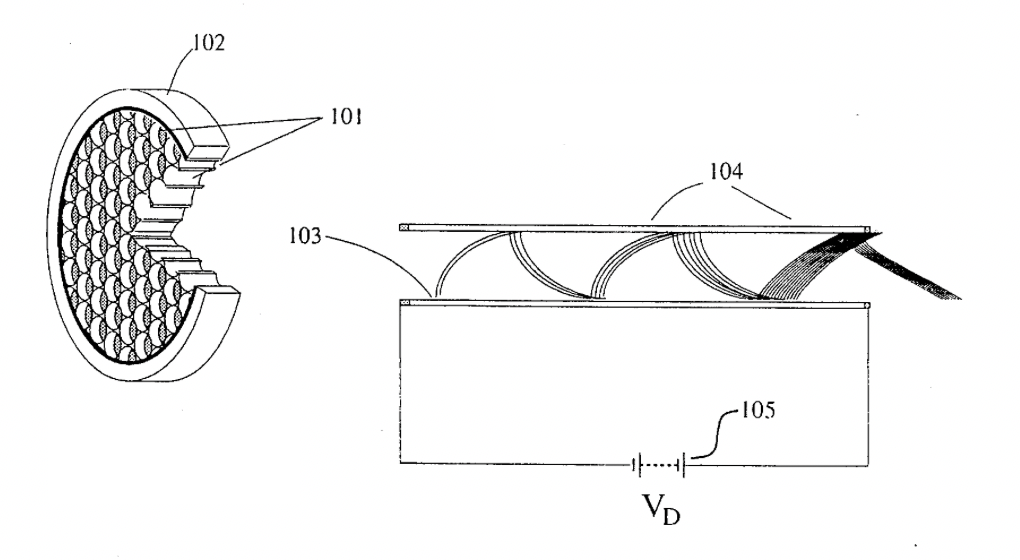
\includegraphics[width=.8\textwidth]{MCP.png}
    \caption[Schnitt und Funktionsprinzip einer MCP]{Schnitt und Funktionsprinzip einer MCP aus \cite{MCP}, hier dargestellt mit einem eintretenden Elektron. (102) Haltungsflange, (101) Mikrokanäle aus Glas, (103) Elektron, welches in den Kanal eintritt, (104) erzeugte Sekundärelektronen, (105) Spannungsversorgung der Platten}
    \label{fig:MCP} 
\end{figure}

Typischerweise werden zwei MCPs hintereinander verwendet, wobei sie um \ang{180} zueinander gedreht sind. Sie befinden sich in einer sogenannten \textit{Chevron}-Konfiguration. Die zweite Platte wird verwendet, um die Verstärkung weiter zu erhöhen und Ionen-Feedback zu minimieren. Ionen-Feedback beschreibt das Zurückfließen von Ionen in die Kammer. Die hohe Anzahl an Elektronen in den Kanälen der MCPs können Restgas ionisieren, welches dann, aufgrund der Beschleunigungsspannung, rückwärts durch die Kanäle in die Kammer gelangen könnte. 

Die auf die Frontplatte angelegte Spannung bestimmt, mit welcher Energie die Ionen auf die Platte treffen. Im Optimalfall sollte sie so einstellt werden, dass die Detektionsrate unabhängig von der Spannung wird. Ziel ist, das alle auf den Dektektor treffenden Ionen genügend Energie haben, um Elektronen auszulösen und somit detektiert zu werden. Abbildung \ref{fig:Frontplattenspannung} zeigt den Zusammenhang von Frontplattenspannung und Detektionsrate, bei konstantem Gasdruck und Elektronenstrahl. Die Abbildung zeigt, dass es nicht möglich ist, mit diesem MCP-Detektor vollständig in der Sättigung zu arbeiten, wenn der empfohlene Spannungsbereich eingehalten wird. Bei der Aufnahme sämtlicher Daten werden im Folgenden möglichst große Spannungen größer 2400 V gewählt, um möglichst viele Ionen nachweisen zu können.

\begin{figure}
    \centering
    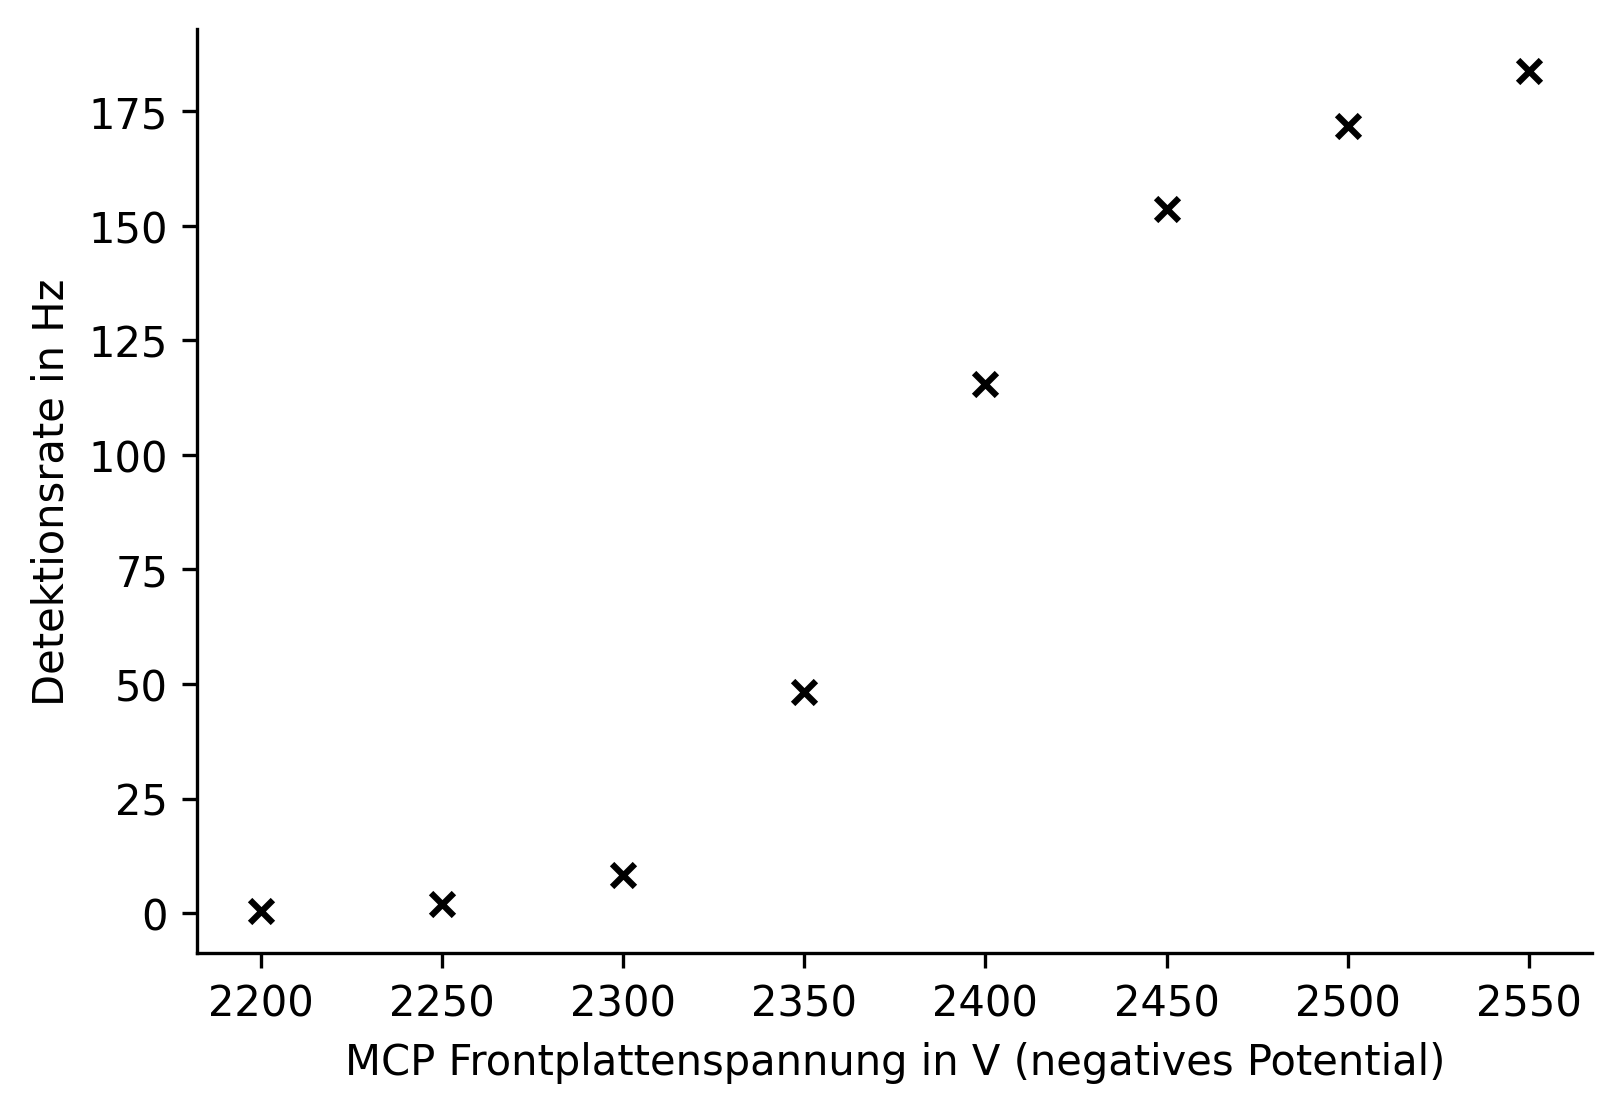
\includegraphics[width=.8\textwidth]{MCP_Sensitivity.png}
    \caption[Detektionsrate in Abhängigkeit der Frontplattenspannung]{Detektionsrate in Abhängigkeit der Frontplattenspannung. Die Rate steigt mit steigender Spannung, bis sie sich bei etwa 2400 V einpendelt.}
    \label{fig:Frontplattenspannung}
\end{figure}

\subsection{Positionsbestimmung}
Wie in \cite{Detektorsystem} dargestellt, gibt es unterschiedliche Ansätze die zweidimensionale Positionsinformation der durch die Platten erzeugten Ladungswolke zu ermitteln. Das Konzept macht sich zu Nutzen, dass eine auf ein Drahtgitter treffende Ladungswolke ein elektrisches Signal in den Leitern erzeugt. Dieses hat eine Laufzeit in der Größenordnung einiger Nanosekunde bis es an den Enden des Leiters ankommt. Anhand dieser Laufzeitdifferenz kann die Position auf dem Detektor in einer Dimension bestimmt werden. Mithilfe eines zweiten, um \ang{90} gedrehten, Leiters, kann die Position zweidimensional dargestellt werden. In Abbildung \ref{fig:DLD} ist die Drahtstruktur für die Messung einer Dimension gezeigt. Der Detektor hat eine aktive Fläche mit einem Durchmesser von 80 mm. In dieser Arbeit ist die Bestimmung der Auftreffpositionen zweitrangig und wird in erster Linie dafür verwendet zu validieren, dass die Ionen tatsächlich primär aus der Elektronenstoßionisation stammen und nicht zufällig verteilt sind. Der Geburtsort der Ionen wird auf dem Bild des Detektors indirekt abgebildet und zeigt deutlich den Strahl der Elektronenkanone. Die Auswertung der Positionsbestimmung erfolgt in in Kapitel \ref{chap:Auswertung}.

\begin{figure}
    \centering
    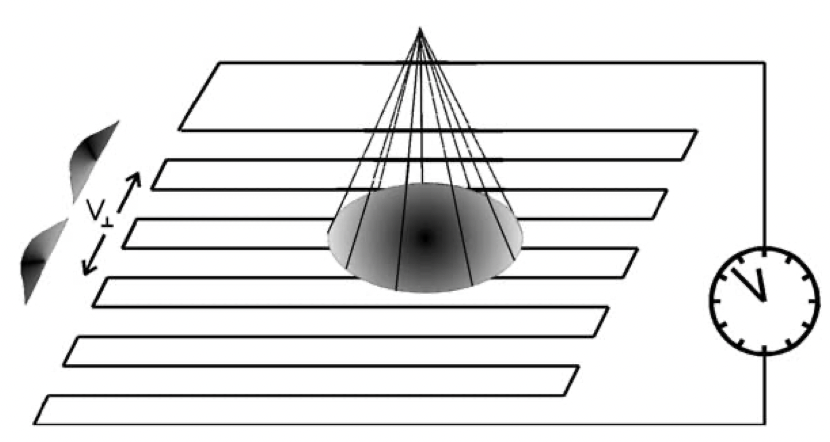
\includegraphics[width=.6\textwidth]{DLD.png}
    \caption[Funktionsprinzip der Laufzeitmessung des Detektors]{Funktionsprinzip der Laufzeitmessung in einer Dimension aus \cite{Detektorsystem}. Der Leiter ist mäanderförmig aufgebaut, um die Laufzeit zu verlängern und die Positionsgenauigkeit zu erhöhen. Das Signal propagiert in beide Richtungen mit der effektiven Geschwindigkeit $v_\perp$.}
    \label{fig:DLD} 
\end{figure}

\section{Konditionierung des Detektors}
Nachdem der Detektor eingebaut ist, muss er einer Konditionierung unterzogen werden, damit er ohne Risiko beschädigt zu werden verwendet werden kann. Zur Konditionierung soll die Spannung zwischen den MCPs in 100 V Schritten erhöht werden und je für einige Minuten konstant gelassen werden. Das hat den Hintergrund, dass Partikel, wie zum Beispiel Staubteilchen, sich von den MCPs oder Teilen des Detektors lösen können und bei schnellem Ansteigen der Spannung Schäden an den Platten hinterlassen können. Beim Konditionieren können diese Partikel sich nach und nach lösen und bekommen nur minimale kinetische Energie zugeführt. Außerdem können Überschläge bei möglichst geringer Potenzialdifferenz festgestellt werden, welche ebenfalls von Partikeln begünstigt werden können. Für die Spannungsversorgung der Detektorplatten wird eine Hochspannungsquelle verwendet, die mit einem Überstromschutz bei sprunghaft ansteigendem Strom abschaltet. Die Konditionierung wird im Vakuum über mehrere Stunden bis zu einer Potenzialdifferenz von 2,7 kV durchgeführt. Nach jedem Erhöhen der Spannung wird der sich eingestellte Strom notiert und der Widerstand berechnet, welcher in etwa konstant bleiben oder sich mit steigender Spannung etwas verkleinern sollte. Tabelle \ref{tab:Konditionierung} im Anhang zeigt die notierten Werte für die Konditionierung ab 880 V, welche ohne Probleme durchgeführt werden konnte. Nach einmaliger Konditionierung kann der Detektor mit einer Geschwindigkeit von etwa 40 V/s ohne weiteres hochgefahren werden.

\section{Signalverarbeitung}
Die auf der Anode des Detektors entstehenden Signale müssen weiterverarbeitet werden, um sie für die Auswertung zu nutzen. Ein Großteil der Signalverarbeitung wird in dieser Arbeit analog umgesetzt. Viele der verwendeten Geräte sind ältere, aber verlässliche Nuclear Instrumentation Module (NIM). Diese können sehr modular in einem Rack verbaut und über BNC-Kabel verbunden werden. Im Folgenden wird die Signalverarbeitung zur Flugzeitmessung und die zur positionssensitiven Auflösung der Ionen unterschieden.

\subsection{Flugzeitmessung}
Eine schematische Übersicht der Verarbeitung ist in Abbildung \ref{fig:ToF} zu finden. Der Signalfluß, angefangen mit dem Startsignal wird nun beschrieben.

\begin{figure} 
    \centering
    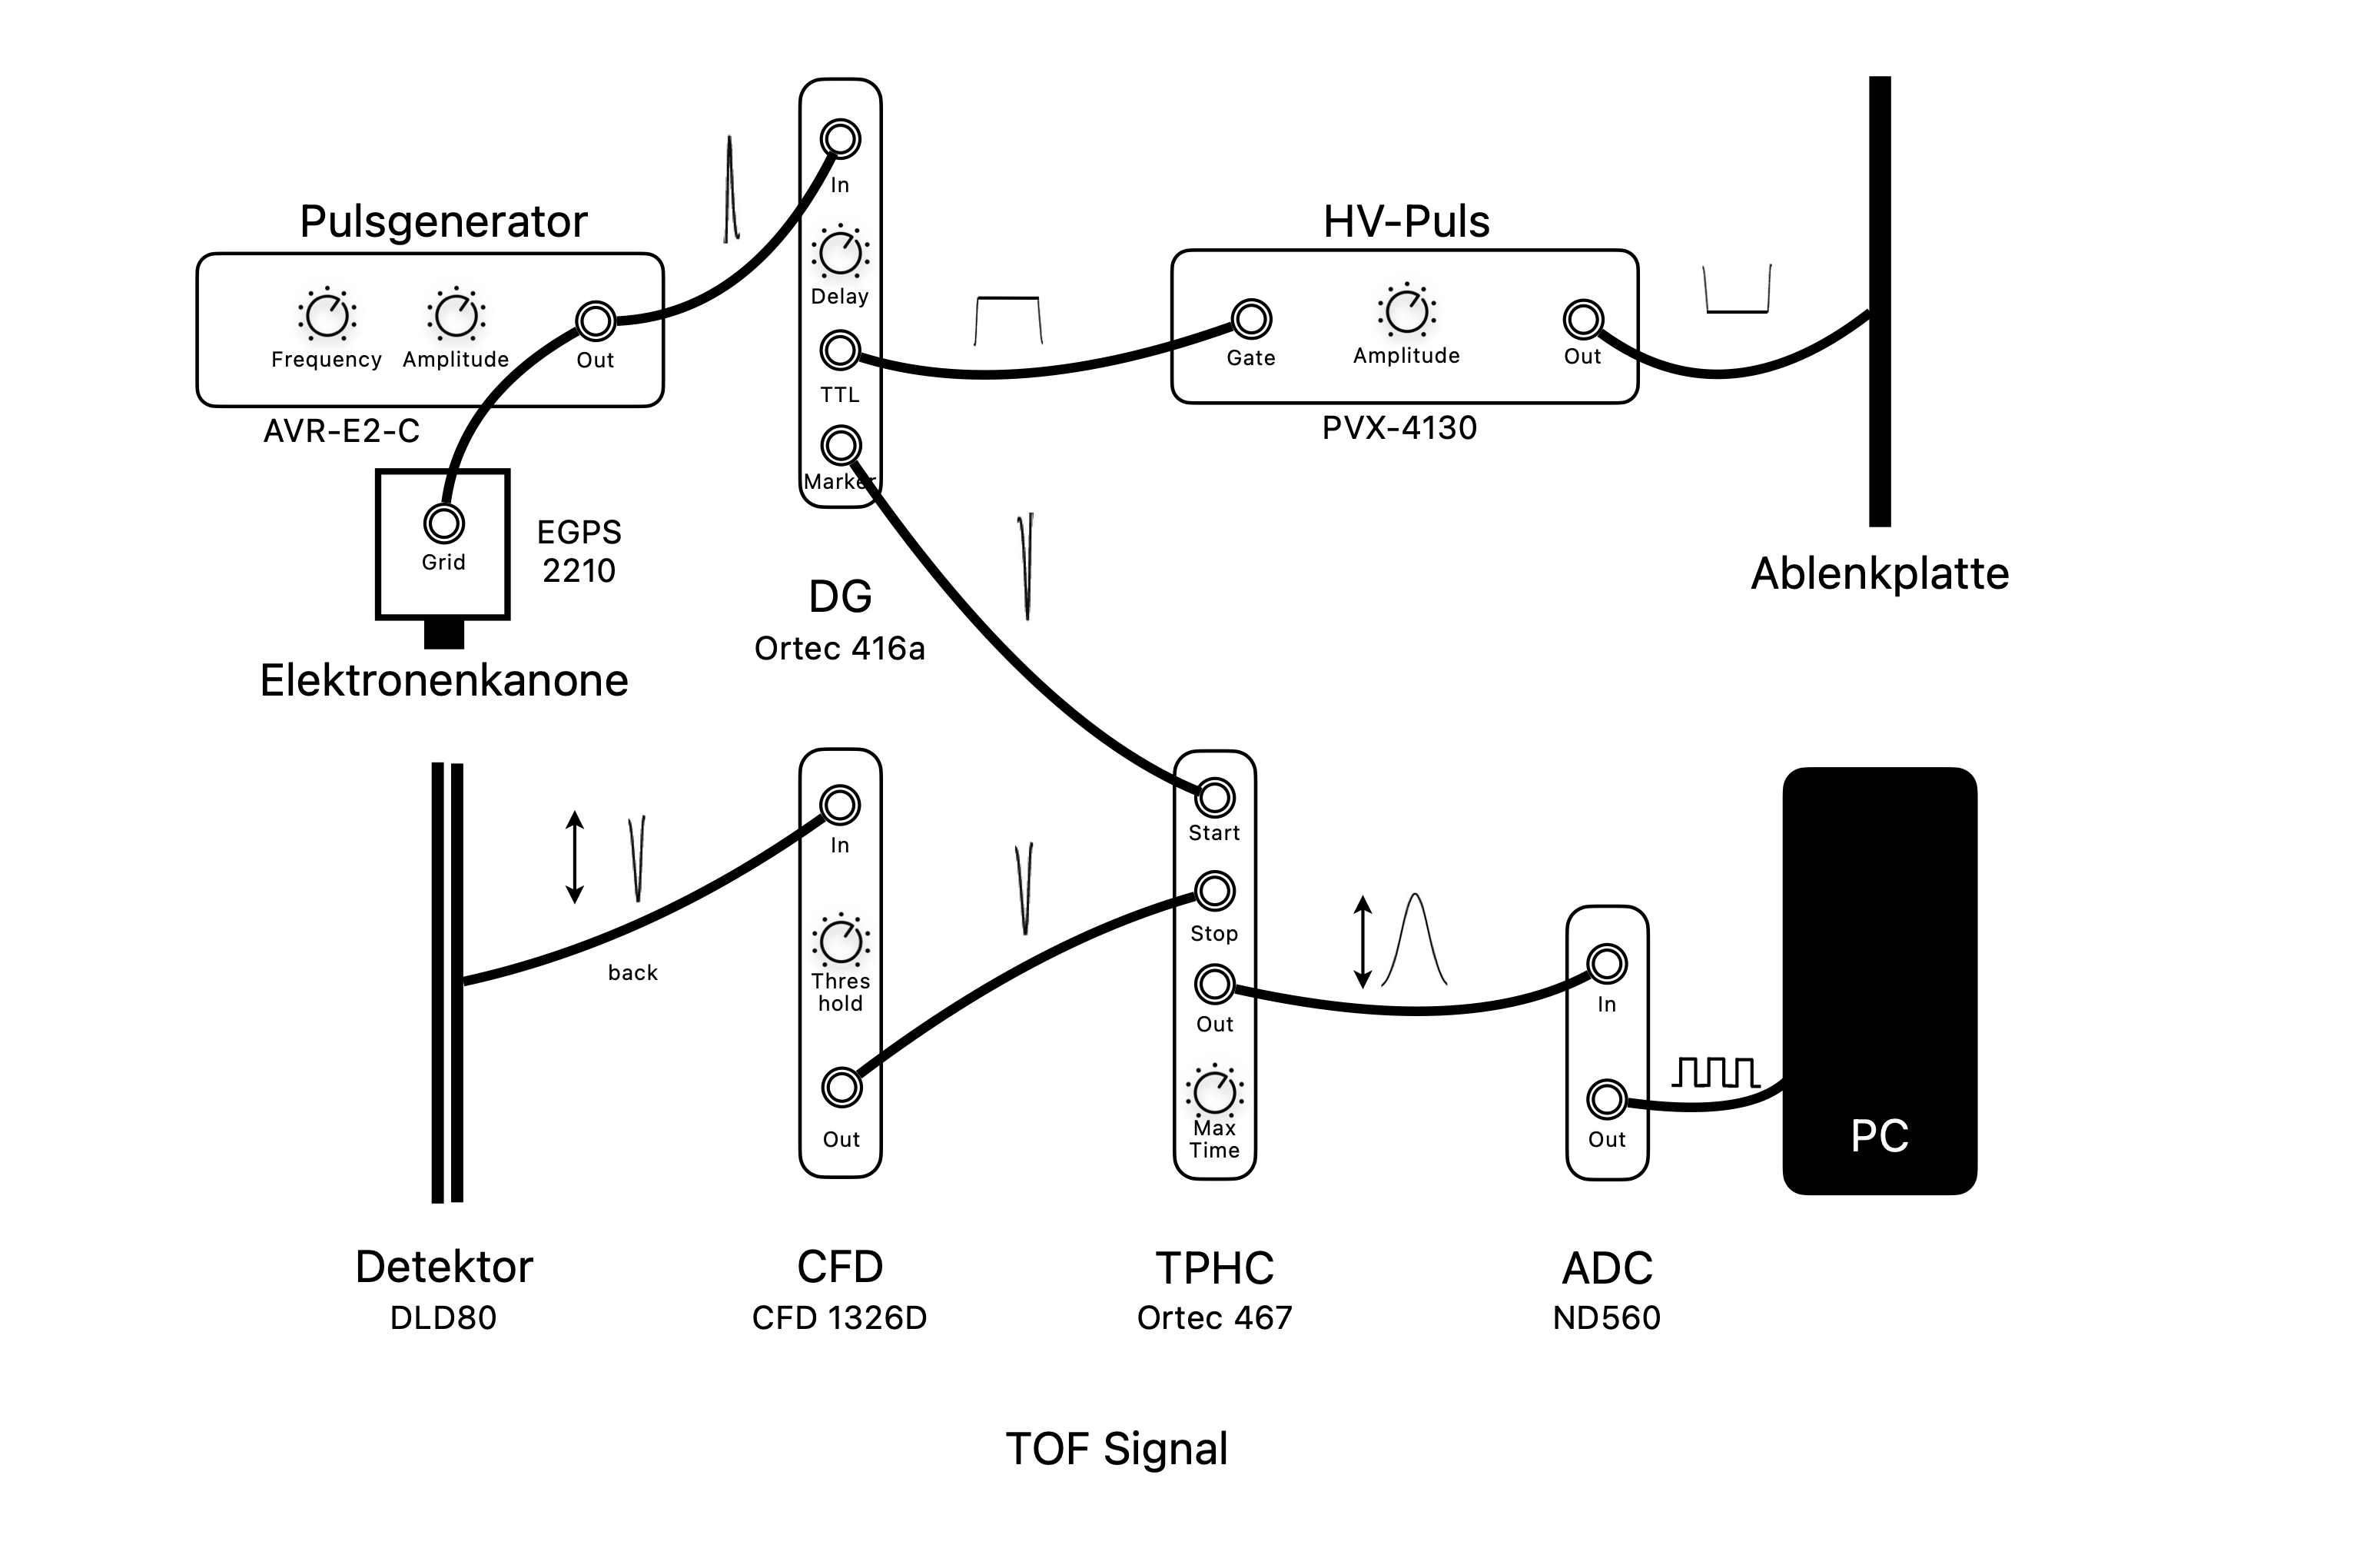
\includegraphics[width=.9\textwidth]{ToF_Signals.png}
    \caption[Schematisch dargestellter Signalfluß der ToF-Messung]{Schematisch dargestellter Signalfluß der ToF-Messung. Der Signalfluß erfolgt, mit Ausname der Elektronenkanone, von links nach rechts. Die verwendeten Geräte sind stark vereinfacht abgebildet, wobei die wichtigsten Einstellungen inkludiert wurden. Die jeweilige Form der Signale ist über den Verbindungen gezeigt und ist rein qualitativ. Power Supplies sowie Anzeigegeräte sind nicht abgebildet.}
    \label{fig:ToF} 
\end{figure}

Um das Startsignal zu erzeugen und die Flugzeitmessung überhaupt in Gang zu setzen, wird ein Pulsgenerator verwendet. Dabei handelt es sich um den AVR-E2-C von AVTECH. Die erzeugten Pulse werden direkt zum triggern der Elektronenkanone verwendet und über einen Delay-Generator (DG) verzögert. Der DG kann sehr genau auf eine Verzögerung einiger Nanosekunden eingestellt werden. Damit ein DG Verzögerungen realisieren kann, wird eine stabile Frequenz benötigt. Diese wird meist durch einen Quarzoszillator erzeugt, ein Kristall über den AC-Pulse angelegt werden. Dieser vibriert mit seiner Resonanzfreuqenz aufgrund des Piezo-Effekts und ermöglicht eine genaue Messung der Zeit. Der TTL-Output des DG wird dann verwendet, um die Ablenkspannung für die Ionen zu erzeugen. Gleichzeitig wird ein Marker (scharfer Puls) ausgegeben, der als Startsignal für die Flugzeitmessung verwendet wird.

Für die Bestimmumg des Auftreffzeitpunktes wird vom Detektor ein Spannungssignal ausgegeben, das von einem Ion beim Auftreffen auf die Anode erzeugt wird.  Der Pegel hängt von der kinetischen Energie des Ions ab und hat eine gewisse Varianz. Der Zeitpunkt soll möglichst unabhängig vom Pegel bestimmt werden können. Wird also lediglich einen Schwellwert (engl. \textit{Threshold}) festgelegt, variert der Zeitpunkt mit der Steilheit der Flanke. Um den Zeitpunkt unabhängig vom Pegel zu bestimmen, wird ein Constant Fraction Discriminator (CFD) verwendet. Dieser erzeugt ein Ausgangssignal, sobald ein bestimmter Bruchteil des Signals erreicht wird. Abbildung \ref{fig:CFD} zeigt das Prinzip des CFD. Dafür wird im CFD das einlaufende Signal verzögert und mit dem Originalsignal über einen Differenzverstärker verrechnet. So ergibt sich ein Nulldurchlauf der Spannung, der von der Verzögerung abhängt, nicht aber von der Amplitude. 

\begin{figure}
    \centering
    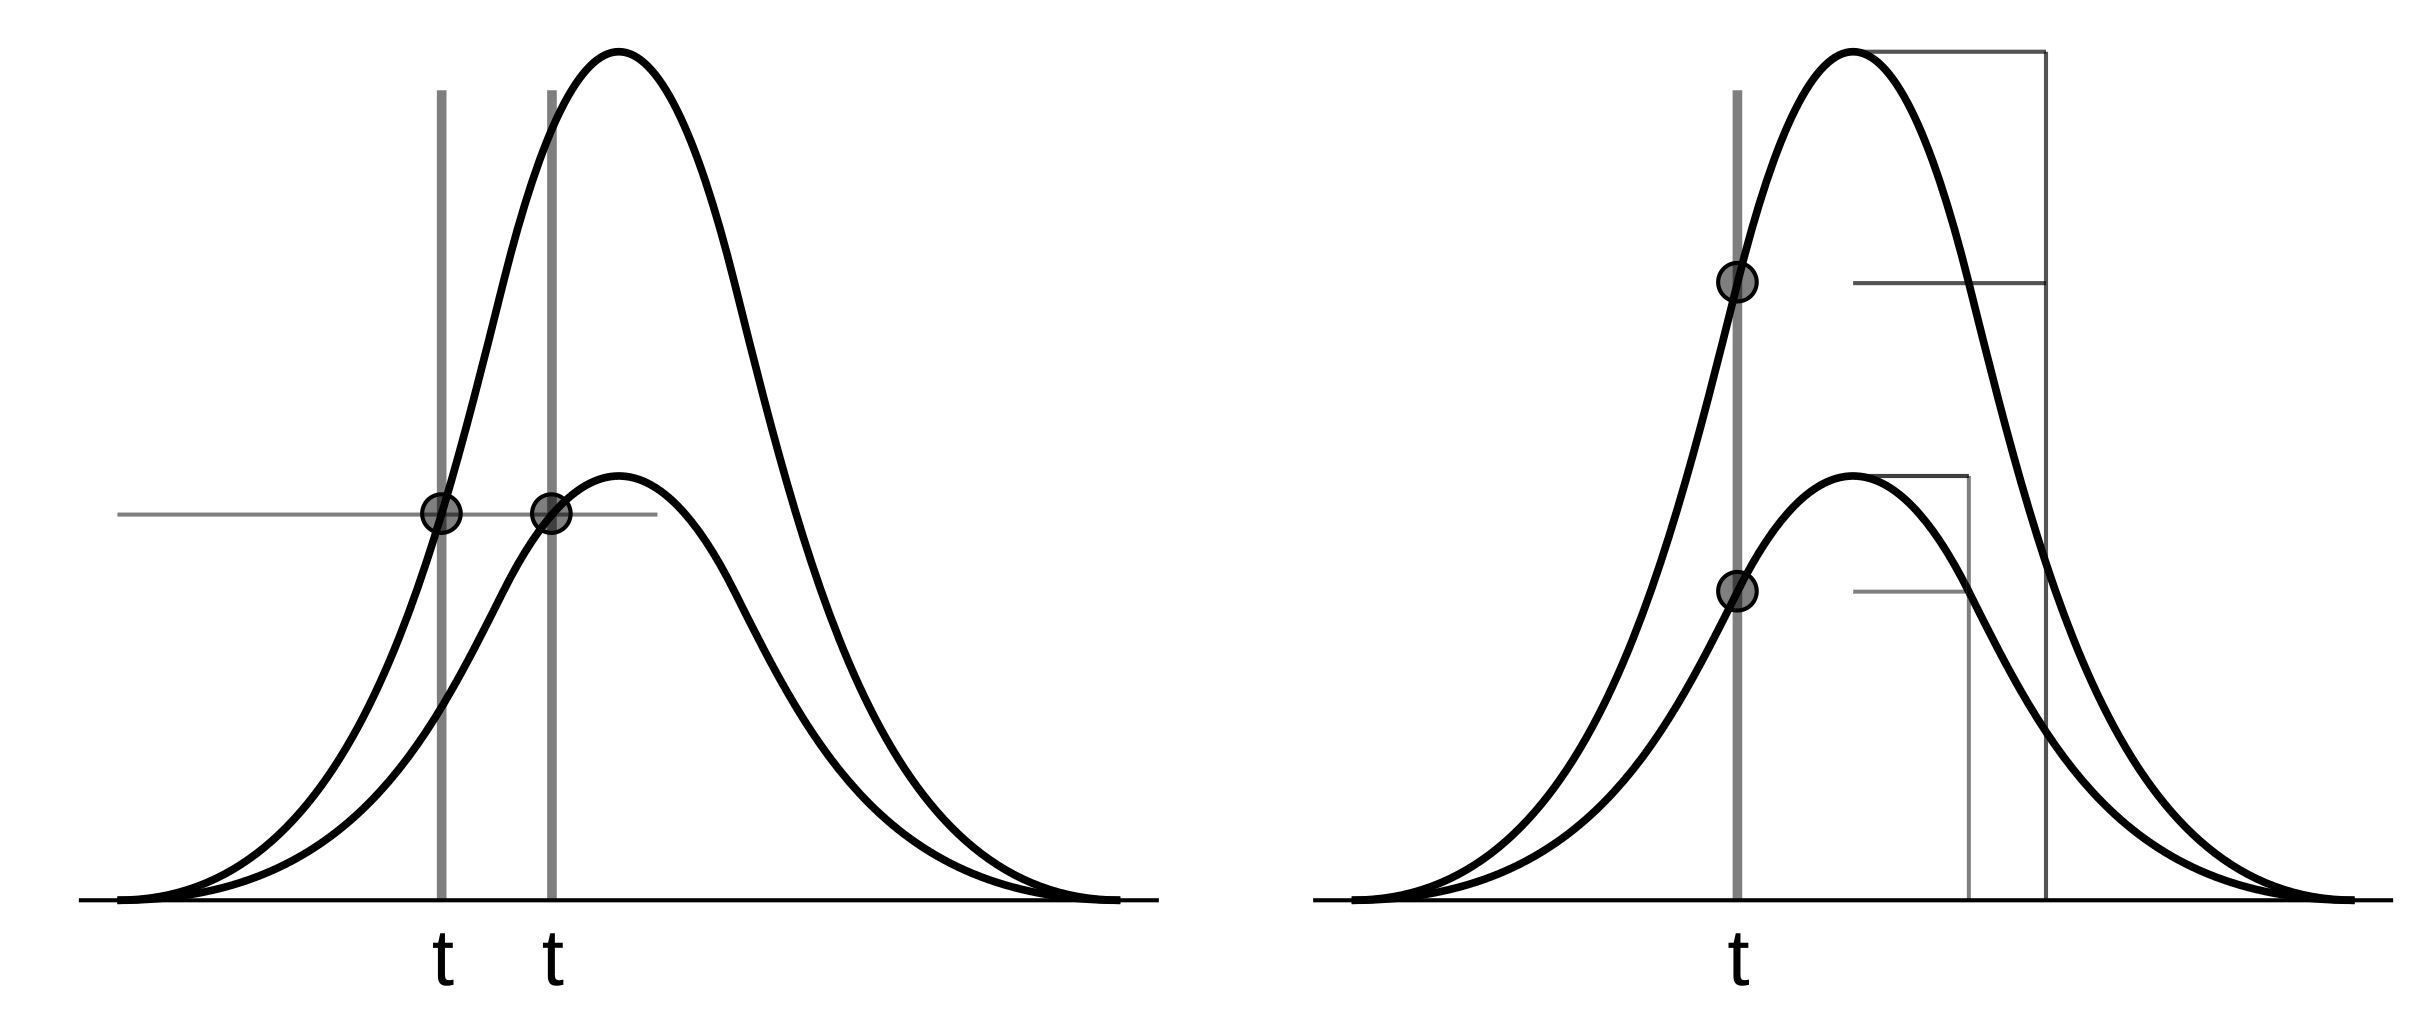
\includegraphics[width=.7\textwidth]{cfd.png}
    \caption[Prinzip des Constant Fraction Discriminators]{Prinzip des Constant Fraction Discriminators. Links: Zeitpunkte beim Überschreiten eines Schwellwertes sind unterschiedlich, rechts: Der Zeitpunkt beim Überschreiten eines Bruchteils des Signals ist unabhängig vom Pegel.\\
    \small Quelle: https://commons.wikimedia.org/w/index.php?curid=534201}
    \label{fig:CFD} 
\end{figure}

Der über den CFD ermittelte Auftreffzeitpunkt kann dann als Stoppsignal für die Flugzeitmessung dienen. Um die Information über die Zeitdifferenz zwischen dem Start- und Stoppsignal zu erhalten, wird ein Time-to-Pulse-Height-Converter (TPHC) Modul verwendet. Dieses erzeugt ein Signal, dessen Höhe proportional zur zeitlichen Differenz eines Start- und Stoppulses ist. Um diese Funktionalität umzusetzen wird im TPHC ein Kondensator aufgeladen, wobei die Spannung über den Kondensator proportional zur Ladezeit steigt. Kommt kein Stoppsignal, wird der Kondensator nach einer eingestellten maximal Dauer über einen Widerstand wieder entladen. Schließlich kann der Spannungspuls über einen Analog-Digital-Converter (ADC) digitalisiert und am Computer ausgelesen werden. Abbildung \ref{fig:Signal} zeigt qualitativ den zeitlichen Verlauf der relevanten Signale der Flugzeitmessung. Anhand vieler Messungen kann ein Spektrum der Flugzeiten erstellt werden.

Dank des Pulsgenerators kann die Messung mehrere tausendmal in jeder Sekunde durchgeführt werden. Begrenzend ist dabei die Elektronenkanone, die, wie bereits erwähnt, mit maximal 5 kHz gepulst werden kann. Für die meisten Messungen wurde eine Frequenz von etwa 3 kHz verwendet.

\begin{figure}
    \centering
    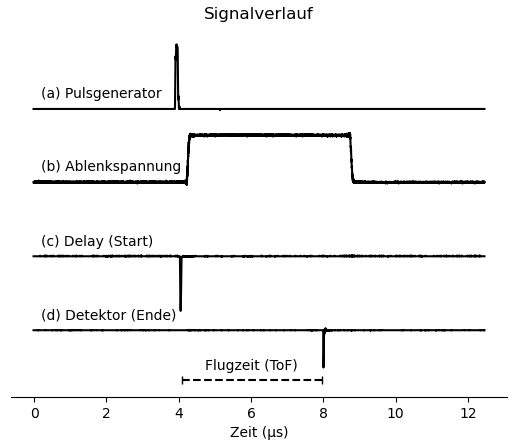
\includegraphics[width=.9\textwidth]{Signalverlauf.png}
    \caption[Aufgenommenener Verlauf der relevanten Signale der ToF-Messung]{Aufgenommenener Verlauf der relevanten Signale. (a) zeigt den initialen Spannungspuls aus dem Pulsgenerator, mit dem auch die Elektronenkanone getriggert wird. Über einen Delay-Generator wird das verspätete Signal (c) erzeugt, um die Ablenkspannung (b) anzusteuern. (d) zeigt das Signal, welches auf der Anode des Detektors entsteht, nachdem es durch den CFD gelaufen ist. Die zeitliche Differenz aus (c) und (d) entspricht der Flugzeit}
    \label{fig:Signal} 
\end{figure}

\subsection{Positionssensitive Auflösung}
In Abbildung \ref{fig:pos} ist der Signalfluß der positionssensitiven Messung schematisch abgebildet und wird nun beschrieben. Die auf dem Drahtgitter entstandenden Signale werden mittels eines Verstärkers von Roentdek verstärkt, wobei darauf geachtet werden muss, dass die Pulse nicht den Verstärker sättigen. Haben die Ionen eine zu große Energie, verliert die Messung der Position an Genauigkeit. Wie auch bei der Verarbeitung der Signale für die Flugzeitmessung wird ein CFD verwendet, um den Zeitpunkt der Signale zu bestimmen. Die analoge Ausgabe des CFD wird dann einem ADC übergeben, der ausgestattet mit der Elektronik von Roentdek die Signale digitalisiert und für die Auswertung am Computer präpariert. Am Computer kann dann das Programm \textit{Cobold} (von Roentdek) verwendet werden, um die von der Hardware ausgelesenen Daten zu visualisieren und zu analysieren. Da die Positionsinformationen nur für die Validierung der Messung verwendet werden, wird auf eine detaillierte Beschreibung der Verarbeitung verzichtet.

\begin{figure}
    \centering
    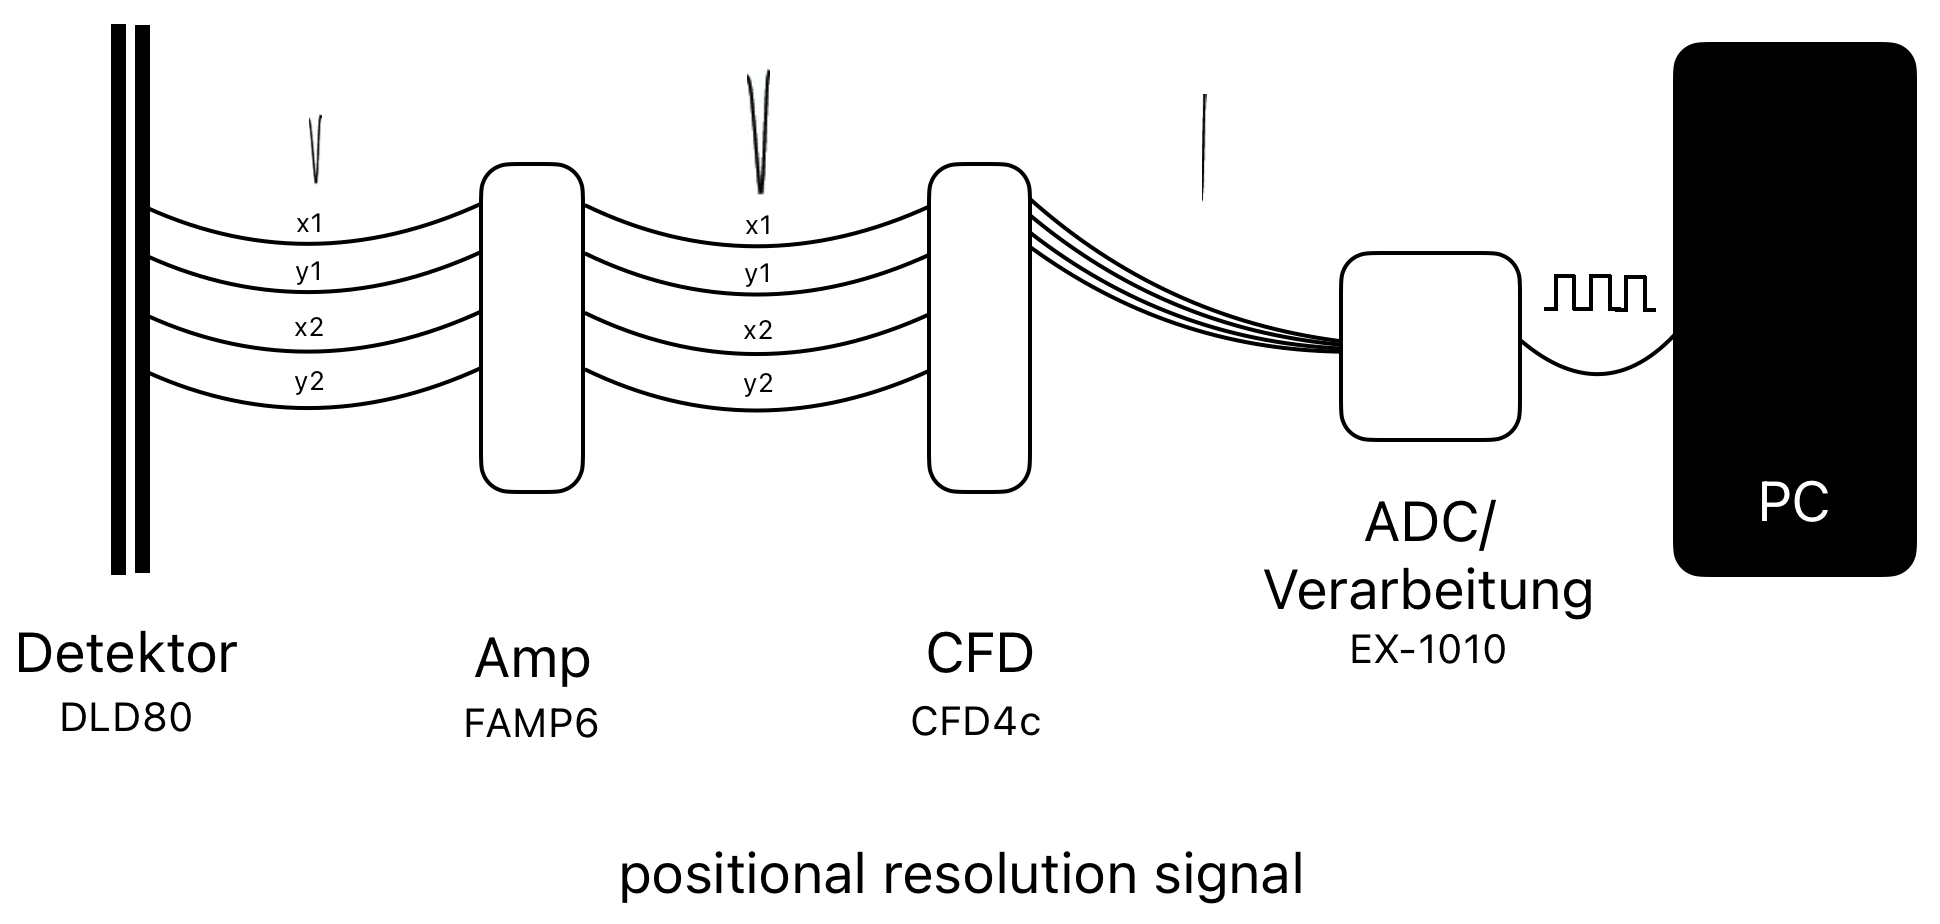
\includegraphics[width=.9\textwidth]{PosSig.png}
    \caption[Signalfluß für die positionssensitive Messung]{Signalfluß für die positionssensitive Messung}
    \label{fig:pos} 
\end{figure}